\section{Privacy Policies}\label{sec-policy}

In Section~\ref{sec-repy}, we introduced the Repy sandbox briefly. 
In this section, we describe how Repy is extended so that experiments
can access smartphone sensors (Section~\ref{sec-repy-ext}), and 
how to control the precision of sensor data (Section~\ref{sec-layer}), 
and frequency of sensor access (Section~\ref{sec-nanny}).

\subsection{Extended Sandbox}\label{sec-repy-ext}

\subsubsection{Sensor Access from the Python Sandbox}

In the use cases in Section~\ref{sec-scenario}, when Alice starts 
the Sensibility Testbed app, the native code in the app initializes a
Python interpreter, launches the Repy sandbox, and starts the 
communication between the device and the clearinghouse. The 
sandbox's API provides calls to file system, networking, 
threading functions, and so on. Therefore, Bob's code can read 
files, send data through the network, etc., from Alice's device. 
Additionally, Bob's code needs access to sensors such as GPS, 
WiFi, Bluetooth, accelerometer, cellular network, etc. To obtain 
such data, we first implemented a set of functions using
Android native code in the Sensibility Testbed app. The Repy 
sandbox then uses a Remote Procedure Call (RPC) to invoke the
corresponding Android code, and returns the data from native code 
to a sandboxed program. This defines a set of sensor API in 
Repy's Python-like language, such as \path{get_location()}, 
\path{get_accelerometer()}, \path{get_wifi()}, etc. 

\begin{figure}
\begin{Verbatim}
1. \textcolor{Purple}{def} \textbf{\textcolor{NavyBlue}{get_location}}():
2.   \textcolor{BrickRed}{"""}
3.   \textcolor{BrickRed}{Get raw location data from GPS, network or passive.}
4.   \textcolor{BrickRed}{"""}
5. 
6.   \textcolor{BrickRed}{# start the locating process} 
7.   sensorlib.request_data(\textcolor{BrickRed}{'startLocating'})
8.
9.   \textcolor{BrickRed}{# try to read current location}
10.  location = sensorlib.request_data(\textcolor{BrickRed}{'readLocation'})
11.
12.  \textcolor{BrickRed}{# stop the locating process} 
13.  sensorlib.request_data(\textcolor{BrickRed}{'stopLocating'})
14.
15.  \textcolor{Purple}{if not} location:
16.    \textcolor{Purple}{raise} LocationNotFoundException    
17.  
18.  \textcolor{Purple}{return} location
\end{Verbatim}
\caption{\small Sandbox implementation of \texttt{get\_location()}. 
\label{fig-getlocation}}
\end{figure}

Figure~\ref{fig-getlocation} shows how \path{get_location()} 
is defined as a sandbox function to get unfiltered location 
information from a mobile device. 
On line 7, \path{sensorlib.request_data()} is an RPC call 
defined in the extended Repy sandbox, 
%\path{sensor_socket} is the socket for the Repy code to communicate with the native code, 
and the string \path{'startLocating'} is the name of the native Java method that tells the Android 
location manager to start to look up location information. Line 10 and 13 are similar RPC 
calls that reads location information from the Android locaiton manager, and stops the location 
lookup. Therefore, \path{get_location()} %is defined in the namespace of the sandbox kernel, it 
can be used by an experimenter in a sandboxed program if no blurring layer is in place.
A full list of sensor
API is documented at~\cite{sensor-api}. As
such, the original Repy interface and the added sensor API together 
provide the complete \textit{OS level} sandbox kernel on a mobile 
device, as shown in Figure~\ref{fig-blur}.

\begin{figure}
\center{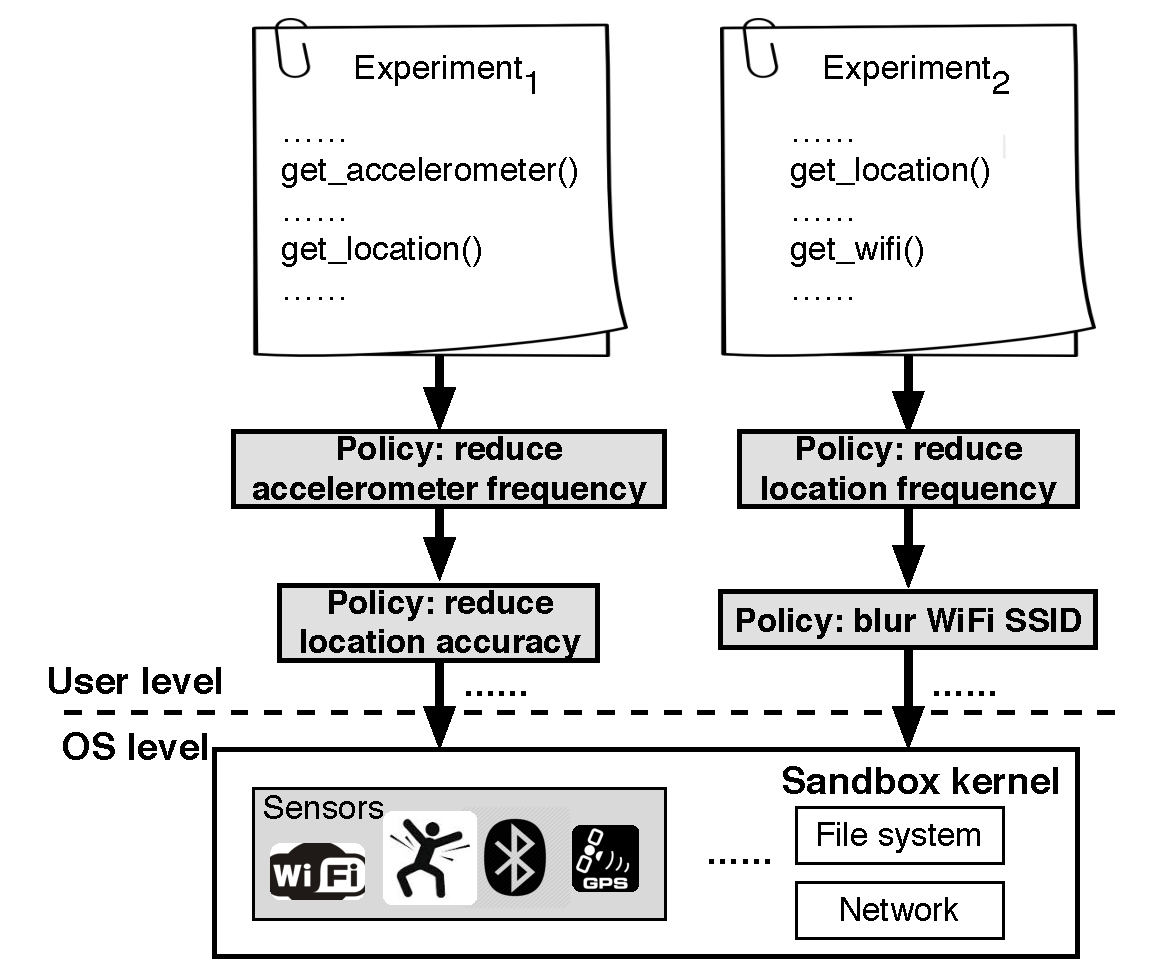
\includegraphics[width=\columnwidth]{figs/blur.pdf}}
%\vspace*{-20pt}
\caption{\small Sensibility Testbed blur policies. \yanyan{maybe replot this}
\label{fig-blur}}
\end{figure}

\subsubsection{Policy Stack}
The sandbox kernel determines how IRB policies are implemented by affecting API calls. It can
interpose on a call and modify the data returned, or control the frequency a call can be made over
a period of time. 
%As mentioned above, Bob provided his IRB policies through our clearinghouse.
Before Bob runs his experiment, the clearinghouse loads the access policies and instructs the sandbox on Alice's device to
restrict sensor access accordingly. 

Using the \path{get_location()} call as an example, 
when Bob's code requests location data from Alice's device, the Repy sandbox first
invokes the location-related Android code (line 10 in Figure~\ref{fig-getlocation}). 
When the location data is returned, Bob's IRB policy
indicates that the returned location coordinates should be blurred to the nearest city to Alice's
device, instead of her actual location. As a result, the sandbox returns an approximate location to
Bob's program. Furthermore, as Bob's IRB policy disallows collecting information about cell tower
IDs, any access to cell IDs is blocked entirely on Alice's device. Similarly, other information
like WiFi SSID can be blurred to a hashed string, the frequency to access an accelerometer or a
gyroscope~\cite{michalevsky2014gyrophone} can be restricted to prevent inferring passwords from the
movement and tilt of the device, and so on. 

As shown in Figure~\ref{fig-blur}, different policies
can be stacked together as a set of filters for different sensors, before a sandboxed program can
access the sensor data. We call all the policies implemented by the sandbox a \textit{policy stack}, 
and the implementation of each policy a \textit{blurring layer}.

\subsection{Blurring Layers: Reducing Data Precision}\label{sec-layer}

%\yanyan{TODO: replace all security layers with blurring layers. fix the line wrapping.}
%The Sensibility Testbed uses an extended version of the Repy sandbox, whose 
%security mechanism is described in our prior work by Cappos, {\it et 
%al}~\cite{cappos2010retaining}. This section briefly explains this sandboxing 
%technique, and how it is used in Sensibility Testbed.

In Sensibility Testbed, we construct a researcher's IRB policies as a set of 
isolated and contained reference monitors called blurring layers. They can 
be stacked together to form a policy stack. A lower layer is the ancestor of 
a higher layer. Each 
blurring layer implements an IRB policy, is untrusted by its ancestor layers, 
but is trusted by its descendant layers. Every layer inherits the policy 
defined by its ancestor layer. The experiment program is on the top 
of the policy stack, therefore it inherits all the policies defined by the
lower layers. The lowest blurring layer with no ancestors is the 
Sensibility Testbed's sandbox kernel, as shown in Figure~\ref{fig-blur}. 

A policy is implemented by each blurring layer via a \textit{virtual 
namespace} that provides a function mapping that substutes raw 
data access with restricted data access. 
%and the boundary between two blurring layers is monitored by an 
%\textit{encasement library} that verifies interface semantics at runtime. 
To ensure the runtime behavior of each function mapping (for example, 
a function mapping of \path{get_location()} still returns location data), 
every blurring layer uses a \textit{contract} to verify the interface 
semantics between the blurring layers.

\subsubsection{Virtual Namespace}

The namespace of each blurring layer executes the code with the 
corresponding layer's function mapping. By our convention, the 
namespace of a blurring layer does not contain functions from the 
sandbox kernel or the namespace of its parent layer, unless explicitly 
specified by the mapping. For example, if a layer \path{foo} with 
functions \path{get_battery()}, \path{restricted_get_accelerometer()}, 
and \path{get_accelerometer()} were to instantiate a descendant 
layer \path{bar} with a function mapping 

\begin{Verbatim}
\{\textcolor{BrickRed}{'get_battery'}: get_battery, 
\textcolor{BrickRed}{'get_accelerometer'}: restricted_get_accelerometer
\}
\end{Verbatim}
then the module \path{bar} would have access
to \path{foo.get_battery} via the name \path{get_battery}, and to
\path{foo.restricted_get_accelerometer} via the name 
\path{get_accelerometer}. In this case, layer \path{bar} would not 
be able to access \path{foo.get_accelerometer}.

\subsubsection{Contract}

%The virtual namespace is useful for loading
%code dynamically, but does not provide adequate security for
%use as an isolation boundary. The encasement library in the 
%Repy sandbox provides isolation between virtual namespaces. 
%Security layers do not share objects or functions.
%The encasement library copies all objects that are passed
%between security layers.
%
Each function call that can be called by descendant blurring
layers needs to be verified of its arguments, return value, and 
other runtime behavior. This concept is similar to system call filtering
mechanisms~\cite{acharya2000mapbox, fraser2000hardening} 
that mediate access to a sensitive function interface. In our case, 
the functions are the calls to smartphone sensors that 
can potentially reveal device owner's private information. The 
verification in our case uses a contract. For each function that needs a 
mapping, the contract lists the number 
and types of its arguments, the exceptions that can be raised 
by the function, and the return type of the function\footnote{Since 
Python is a dynamically typed language, it is useful to type check 
a function's arguments, exceptions, and return values.}.

A contract is represented as a Python dictionary. As an example, if 
the blurring layer \path{foo} wanted to create a contract that would map
\path{get_battery{}} and \path{restricted_get_accelerometer()} into 
a new namespace, the contract would be: 

\begin{Verbatim}
\{\textcolor{BrickRed}{'get_battery'}: \{
  \textcolor{BrickRed}{'type'}: \textcolor{BrickRed}{'func'},
  \textcolor{BrickRed}{'args'}: \textcolor{Purple}{None}, 
  \textcolor{BrickRed}{'exceptions'}: (\textcolor{Purple}{BatteryNotFoundError}), 
  \textcolor{BrickRed}{'return'}: dict,
  \textcolor{BrickRed}{'target'}: get_battery
  \}, 
\textcolor{BrickRed}{'get_accelerometer'}: \{
  \textcolor{BrickRed}{'type'}: \textcolor{BrickRed}{'func'},
  \textcolor{BrickRed}{'args'}: str, 
  \textcolor{BrickRed}{'exceptions'}: (\textcolor{Purple}{ValueError}), 
  \textcolor{BrickRed}{'return'}: list,
  \textcolor{BrickRed}{'target'}: restricted_get_accelerometer
  \}
\}
\end{Verbatim} 

Note that the symbols in the contract come from \path{foo}'s 
namespace. Thus the target for the \path{get_battery} in the 
contract is the \path{foo.get_battery} function. Similarly, the 
target for the \path{get_accelerometer} in the contract is the 
\path{foo.restricted_get_accelerometer}.

Whenever a function is called, the verification process uses the 
contract to perform type-checking. If the verification process 
detects a semantic violation, the entire experiment program is 
terminated. 
%In addition to type checking, the verification function copies 
%arguments and return values of mutable types to prevent 
%time-of-check-to-time-of-use bugs. Since mutable types are 
%copied, the caller cannot cause a race condition by modifying objects.

\subsubsection{Blurring Layer Instantiation}

Each blurring layer provides a contract to instantiate the 
next blurring layer by substituting a version of the function that 
enforces a given policy. All descendant layers (layers loaded 
after this layer) will have access to the version of the function 
which enforces this new policy. The final blurring layer starts the 
experiment program with the appropriate set of functions. 
Therefore, the experimenter's program is forced to use all the 
new policies. An example blurring layer implementation is given in 
Section~\ref{sec-precision-example}.  

From start to finish, the entire process proceeds as follows. 
The clearinghouse creates a list of access policies for an experimenter's
experiment, according to the IRB policies specified by this 
experimenter. The sandbox on a mobile device (under the control of
this researcher) obtains a list of command-line arguments 
from the clearinghouse, which includes all the blurring layers.
%the first of which must be the encasement library.
%The kernel reads in the encasement library code and uses
%the virtual namespace abstraction to execute the code with
%the exported kernel functions. The encasement library
The sandbox then uses its blurring layer creation call to instantiate 
the first blurring layer according to its contract (or the function 
mapping that contains the kernel's exported functions).
%the security layer instantiation call, and the remaining
%command-line arguments. 
The newly instantiated blurring layer repeats this process using the 
%encasement library's
blurring layer creation call to instantiate the next
security layer with a potentially updated contract and function
mapping. Eventually, the experimenter's program is instantiated
in a separate security layer with the functions provided
through the stack of blurring layers that preceded it.
The experimenter's program will then be subject to all the 
policies defined in the preceding layers.

\subsubsection{An Example Policy Implementation}
\label{sec-precision-example}

%\subsubsection{Reducing Data Precision}

The following is an example implementation of a location blurring layer. 
When experimenter Bob requests a device, the clearinghouse recognizes that all the location data
collected by Bob must be substituted with a blurred location that only identifies a nearest city.
%rather than the exact location of the device. 
Therefore, the following blurring layer is
automatically loaded along with Bob's experiment code, to map 
the \path{get_location()} call in Figure~\ref{fig-getlocation} to a version 
that implements such a policy. \yanyan{load code or load policy text? how
to translate policy text to code?}In the following, we name this
blurring layer \path{blur_to_city}, and assume it is the first descendant
of the sandbox kernel.

\begin{Verbatim}
1. \textcolor{Purple}{def} \textbf{\textcolor{NavyBlue}{get_city_location}}():
2.   \textcolor{BrickRed}{"""}
3.   \textcolor{BrickRed}{This function replaces the exact coordinates of} 
4.   \textcolor{BrickRed}{the Android device with the coordinates for the } 
5.   \textcolor{BrickRed}{geographic center of the nearest city.}
6.   \textcolor{BrickRed}{"""}
7.
8.   location = get_location()
9.
10.  closest_city = find_closest_city(location[\textcolor{BrickRed}{"latitude"}],
11.    location[\textcolor{BrickRed}{"longitude"}])
12.
13.  location[\textcolor{BrickRed}{"latitude"}] = closest_city[\textcolor{BrickRed}{"latitude"}]
14.  location[\textcolor{BrickRed}{"longitude"}] = closest_city[\textcolor{BrickRed}{"longitude"}]
15.
16.  \textcolor{Purple}{return} location
17.
18. \textcolor{BrickRed}{# Substitute get_location with get_city_location.}
19. \textbf{CHILD_CONTEXT_DEF[\textcolor{BrickRed}{"get_location"}] = \{}
20.    \textbf{\textcolor{BrickRed}{"type"}: \textcolor{BrickRed}{"func"},}
21.    \textbf{\textcolor{BrickRed}{"args"}: \textcolor{Purple}{None},}
22.    \textbf{\textcolor{BrickRed}{"return"}: \textcolor{Purple}{dict},}
23.    \textbf{\textcolor{BrickRed}{"exceptions"}: \textcolor{BrickRed}{"any"},}
24.    \textbf{\textcolor{BrickRed}{"target"}: get_city_location,}
25. \textbf{\}}
26.
27. \textbf{secure_dispatch_module()}
\end{Verbatim}


Line 1 -- 16 defines a new function \path{get_city_location()} which returns 
a nearest city to the device. 
%in \path{blur_to_city}'s namespace that is outside the sandbox kernel. 
Lines 19 -- 25 defines a contract for \path{get_city_location()}. 
%and stores it in a global dictionary \path{CHILD_CONTEXT_DEF}. 
The target for \path{get_city_location()} in this
contract is the sandbox kernel function \path{get_location()} (line 19).
This means that \path{get_city_location()} will substitute  
\path{get_location()} defined by the sandbox.
%On Line 19, \path{CHILD_CONTEXT_DEF} indicates that this data structure is to replace the
%Repy library function \path{get_location()}. 
Line 20 - 23 define the function's type, arguments,
return values, and any potential exceptions for runtime verification. 
%Line 24 indicates that Repy library function
%\path{get_location()} will be replaced by \path{get_city_location()} defined in line 1 - 16, once
%this blurring layer is in effect, which means the blurring layer is enforced via running along a
%sandboxed program. Finally, in order for this blurring layer to take effect, we need to call
Finally, \path{secure_dispatch_module()} (line 27) instantiates this
\path{blur_to_city} layer, when running along with the sandbox kernel. 
\yanyan{or does it instantiate experiment code?}As a result, 
whenever Bob's experiment code calls \path{get_location()} defined in the sandbox, 
the \path{blur_to_city} layer replaces it with \path{get_city_location()}. 

Similarly, if Bob's IRB policy disallows access to cell ID, then another blurring layer 
can substitue the \path{get_cellID()} call in the sandbox kernel with a function that
returns \path{None}. %This layer can be instantiated by any other layers.
Such a policy implementation is opaque to all the experimenters who run 
sandboxed programs in Sensibility Testbed.

\subsection{Nanny: Restricting Data Access Frequency}\label{sec-nanny}

Reducing data precision partially protects a device owner's privacy. Frequent data 
access can also be another channel for a program to snoop personal information.
Additionally, the battery power of a device can be drained if sensors are accessed
unnecessarily frequently. The sandbox in Sensibility Testbed provides a second mechanism
called \path{nanny}, to mediate and restrict the access frequency to sensors. 

\subsubsection{Access Regulation}

\path{nanny} treats all sensors as \textit{resources}, and the function calls to 
access the sensors as the \textit{usage} of resources. \path{nanny}'s control 
mechanism for a resource is to limit the \textit{rate} of its usage. For example, 
when an 
%Utilization is controlled over one or more periods, where
experiment program's use of the resource is above a given threshold, the 
program is paused for as long as required to bound it below the
threshold, on average. Therefore, if an experiment program attempts to 
use a resource at a rate faster than is allowed, the function 
call to a sensor is blocked until sufficient time has passed. 

To monitor and control the usage of resources, \path{nanny} keeps a 
table of resource assignments that track and update requests and releases. 
Once resource caps are set, an experiment program can never call a 
function to access a sensor more frequenly than the cap. A function call 
request can be met only if the frequency is no greater than the cap. 

\subsubsection{An Example Policy Implementation}\label{sec-rate-example}

Since access regulation is a policy, it can also implemented as a blurring layer, 
in a similar way as reducing the data precision (Section~\ref{sec-precision-example}).
Recall that in Section~\ref{sec-irb-policy}, Bob's IRB policy requires that
his experiment can get location updates every 10 minutes (600 seconds). 
Therefore, the following blurring layer is automatically loaded along with 
Bob's experiment code. In the following, we name this blurring layer 
\path{restrict_location}.

\begin{Verbatim}
1.  \textcolor{BrickRed}{# allow get_location call once per 600 seconds}
2.  \textbf{resourcesdict = \{\textcolor{BrickRed}{'get_location'}: 1/600\}} 
3.
4.  \textbf{nanny.start_resource_nanny(resourcesdict)}
5.
6.  \textcolor{Purple}{def} \textbf{\textcolor{NavyBlue}{restricted_get_location}}():
7.    \textbf{nanny.tattle_quantity(\textcolor{BrickRed}{'get_location'}, 1)}
8.    location_data = get_location()
9.    return location_data
10.
11. CHILD_CONTEXT_DEF[\textcolor{BrickRed}{"get_location"}] = \{
12.   \textcolor{BrickRed}{"type"}: \textcolor{BrickRed}{"func"},
13.   \textcolor{BrickRed}{"args"}: \textcolor{Purple}{None},
14.   \textcolor{BrickRed}{"return"}: \textcolor{Purple}{dict},
15.   \textcolor{BrickRed}{"exceptions"}: \textcolor{BrickRed}{"any"},
16.   \textcolor{BrickRed}{"target"}:  restricted_get_location,
17. \}
18. 
19. secure_dispatch_module()
\end{Verbatim}

Line 2 above defines the resrouce assignment table to track and update 
the function call to \path{get_location()}. Line 4 initializes \path{nanny} 
with the resrouce assignment table, and line 6 -- 9 defines a 
function \path{restricted_get_location()} that restricts locaiton updates. 
The \path{tattle_quantity()} call on line 7 charges \textit{one} \path{get_location()} call 
request. It tells \path{nanny} that when \path{restricted_get_location()} 
is called, \path{get_location()} (line 8) will be called exactly once. The
next time this experiment program 
%calls \path{get_location()} again, the program 
will be paused for 600 seconds before it can call \path{get_location()} again.

The contract on line 11 -- 17 defines that the target
for \path{restricted_get_location()} is \path{get_location()}. If 
\path{restrict_location} is the first descendant of the sandbox kernel, then
\path{restricted_get_location()} will replace the \path{get_location()}
in the sandbox virtual namespace. If there is a preceding blurring layer 
before \path{restrict_location} that already updated its 
function mapping for \path{get_location()} (like \path{blur_to_city}  
in Section~\ref{sec-precision-example}), then
\path{restricted_get_location()} will replace the \path{get_location()} call
with the policy implemented in this preceding blurring layer.

\smallskip
The mechanisms in this section are all transparent to the experimenters 
and device owners, as the implemetation of policies is controlled by the 
clearinghouse on behalf of the experimenters. An experimenter is aware 
of a certain policy in place, but does not need to explicitly invoke such a 
policy. 